\section{AutoMArch}
AutoMArch is capable of creating multi-threaded in-order designs of any number of threads and any number of pipeline stages that is functionally equivalent to n-copies of the input base functional datapath, where n is the number of threads. The functionality of the input base datapath is defined by its input output behavior and its next state update behavior. Two designs are defined as functionally equivalent if given the same starting architectural state and sequence of inputs, the two designs transition to the same ending architectural state and produce the same sequence of outputs. Architectural state elements are defined as the state elements present in the input base functional datapath. AutoMArch always preserves the state elements present in the input base functional datapath, but maybe add additional state elements such as pipeline registers that are not considered architectural state.

\subsection{Input Datapath Restrictions}
The input base functional datapath can be an arbitrary FSM with the following restrictions:

{\bf (1)} The input FSM must communicate to the outside world through ready/valid ports  

{\bf (2)} The designer cannot use input valid or output ready signals as inputs to any part of their circuit

{\bf (3)} Any functional units that may take more than one clock cycle to return responses(caches, multipliers, dividers, etc) must be accessed through the Variable Latency Unit Interface discussed below.

Condition {\bf (1)} is necessary because the transformed design will have different input to output latency than the original design depending on what stages the input and output ports are placed in the pipeline. Additionally, some pipeline stages may contain bubbles or be stalled and it would be incorrect to receive inputs or produces outputs under these conditions. Thus by enforcing that only ready/valid IO ports are used, correct IO behavior can be defined by only the sequence of valid inputs tokens accepted and sequence of valid outputs tokens produced, without any restriction on the exact timing of when the input tokens are accepted and output tokens are produced.

\subsubsection{IO Semantics}
When input ready or output valid is driven high by the input FSM, this implicity signals to the tool that the input FSM requires the use of the input or output port on the current state update. Thus, the tool generates logic that examines the input ready or output valid and stalls the pipeline if the corresponding input valid or output ready is not driven high by external modules. The designer should design the input FSM so that input readies and output valids are only driven high when absolutely necessary to avoid unnecessary stalling the automatically multi-threaded and pipelined version of the circuit.

\begin{figure}
	\centering
    \resizebox{\columnwidth}{!}{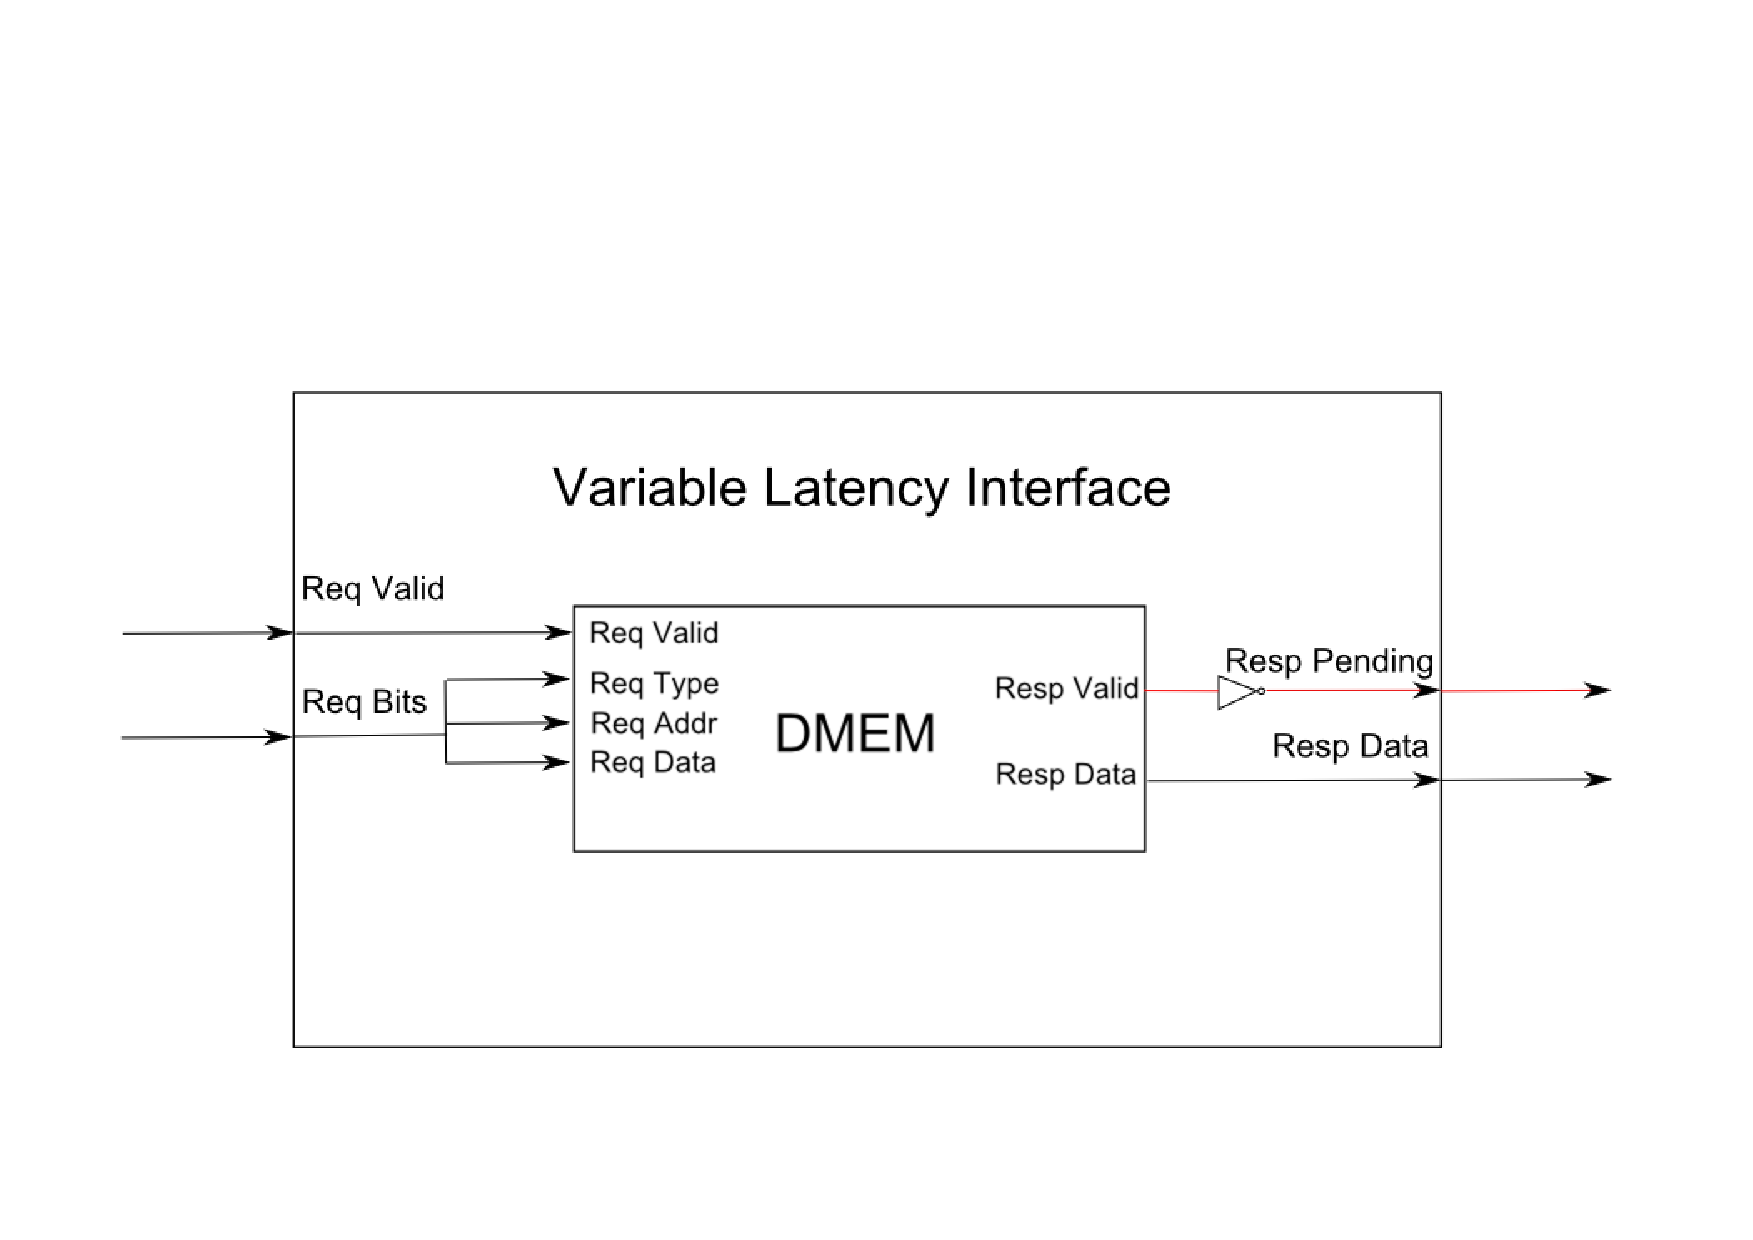
\includegraphics{figures/TransactionalInterface}}
    \caption{{\bf Single Thread View of Variable Latency Unit Interface} Black wire are user facing IO, red wires are tool facing IO}
	\label{fig:VarLatIO}
\end{figure}

\subsubsection{Variable Latency Unit Interface}
In order to accomodate caches and long latency arithmetic units in the minimal FSM specification that is not allowed to have any optimization or control logic implemented, the tool provides the Variable Latency Unit Interface. The designer should access any caches or long latency arithmetic units through a Variable Latency Unit Interface and treat that Variable Latency Unit Interface like a piece of combinational logic in the input FSM specification. IE the designer should not use the Resp Pending port of the Variable Latency Unit Interface to drive any part of their circuit and should pretend that the Variable Latency Unit Interface always gives a valid response immediately. The tool will automatically generate control logic that deals with the Variable Latency Unit Interface not immediately outputting a valid response.

\subsection{Conventions}
{\bf State Element Partitioning}
State elements in the input FSM will be considered as multiple circuit components. For singular registers, the read output is considered a separate component from the write data and write enable inputs and will be referred to as the register's read port. The write data and write enable input is considered together as a single circuit component and will be referred to as the register's write port. For memories, which could be either an array of registers or a SRAM block, each read port and each write port is considered a separate component. 

This partitioning of the state elements into separate read and write ports make it easier for AutoMArch to analyze the input datapath because it allows the datapath to viewed as a acyclic circuit component graph in which data flows from the state element read ports and input pins through combinational logic nodes into the state element write ports and and output pins.

{\bf Pipeline Terminology}
Traditionally, in order pipelining is discussed with regards to processors or stateless combinational units. Pipelining stateless combinational units is trivial as there are no inter-pipeline stage dependencies. When pipelining processors, we consider the dependencies between each instruction flowing down the pipeline when creating pipeline control logic. However, pipelining as discussed in this thesis can be applied to arbitrary finite state machines. In this context, it does not make sense to talk about instruction to instruction dependencies as we are not only dealing with arbitrary FSMs. Instead, we will consider there to be a series of next state updates flowing down the pipeline. When constructing pipeline control logic, we will consider dependencies between each next state update flowing down the pipeline.

\subsection{Automatic Pipelining}
\subsubsection{Pipelining Options}
First the designer must select the number of pipeline stages the optimized design should have. This is the minimum specification needed. If no additional specification is provided, the tool will automatically place all of the pipeline registers and default to generating an inorder pipeline that resolves all pipeline hazards by interlock.

{\bf Pipeline Stage Placement}
By default, the tool places all of the architectural state element read ports in the first pipeline stage and the architectural state element write ports along with the output ready/valid ports in the last pipeline stage. The tool then automatically place the rest of the circuit components in a pipeline stage that minimizes the critical path delay.

If this default placement is not suitable, the designer is given the option to manually place specific circuit components. For example, in a RISC processor design, the PC register write port should be placed as early as possible in the pipeline to minimize branch penalty. The designer does this by annotating circuit components with the desired stage number in the RTL source file of the base functional datapath. Then when the tool does the automatic placement of the circuit components, it will first place the user annotated components in their specified pipeline stage before it automatically places the rest of the unannotated circuit components. 

Thus, the designer has the flexibility to manually place none, some, or all of the circuit components in the base functional datapath. The designer can initially let to the tool place all of the circuit components and gradually manually place components as performance issues are discovered.

{\bf Pipeline Hazard Resolution}
In the traditional framework of inorder processor pipeline design, there are three types of hazards - data hazards, control hazards, and structural hazards. Only data hazards need to be dealt with by the tool. Data hazards arise when the next state update in pipeline stage X reads a state element that could be written by a next state update in pipeline stage Y, where Y > X, but Y <= the stage of the state element's write port. In traditional pipelined processors, control hazards arise when the next PC information is not available soon enough for branch and jump instructions. This is really just a data hazard on the PC register and does not need to be considered separately. Likewise, in traditional pipelined processors structural hazards arise when instructions in different stages of the pipeline need to write to the register file at the same time, but there is only one register file write port. This cannot happen in AFDO because the input base functional datapath does not have multiple pipeline stages and the tool will not generate logic to have instructions at different pipeline stages write to the same architectural state element write port.
\subsubsection{Pipeline Register Placement}
{\bf Legal Placement}
{\bf Optimal Placement}
\subsubsection{Pipeline Control Logic Generation}
\subsubsection{Differences From VLSI Retiming}
\subsection{Automatic Multi-threading}
